\graphicspath{ {assets/cap3/es_2/} }

Il seguente codice MatLab, contiene l'implementazione di una funzione per la \textit{fattorizzazione} $LDL^t$ di una matrice \textit{A}\\\
\begin{itemize}
	\item \textbf{Metodo fattorizzazione $LDL^t$}
	      \lstinputlisting[language=Matlab]{Cap_3/Es_2/fattorizzazioneLDLt.m}
\end{itemize}
Il seguente codice MatLab, contiene la chiamata della funzione precedente :\\\
\lstinputlisting[language=Matlab]{Cap_3/Es_2/Es_2.m}
con i seguenti parametri di input :\\\
\begin{enumerate}
	\item
	      \[
	      	A_1 =\begin{bmatrix}
	      	1  & -1  & 2   & 2  \\ 
	      	-1 & 5   & -14 & 2  \\
	      	2  & -14 & 42  & 2  \\
	      	2  & 2   & 2   & 65 
	      	\end{bmatrix}
	      \]\\
	\item
	      \[
	      	A_2 =\begin{bmatrix}
	      	1  & -1  & 2   & 2   \\ 
	      	-1 & 6   & -17 & 3   \\
	      	2  & -17 & 48  & -16 \\
	      	2  & 3   & -16 & 4   
	      	\end{bmatrix}
	      \]\\
\end{enumerate}
restituendo i seguenti risultati:\\\
\begin{enumerate}
	\item
	      $A_1$ è fattorizzabile $LDL^t$\\
	      \[
	      	LDL^t_1 =\begin{bmatrix}
	      	1  & -1  & 2   & 2  \\ 
	      	-1 & 4   & -14 & 2  \\
	      	2  & -3  & 2   & 2  \\
	      	2  & 1   & 5   & 7 
	      	\end{bmatrix}
	      \]
	      E' quindi \textit{sdp}.\\
	\item
	      $A_2$ non è fattorizzabile $LDL^t$, quindi non è \textit{sdp}.
	      Dagli screenshot dell'esecuzione vediamo che al 2° ciclo il programma stabilisce che $A_2$ non è fattorizzabile $LDL^t$:
	      \[ 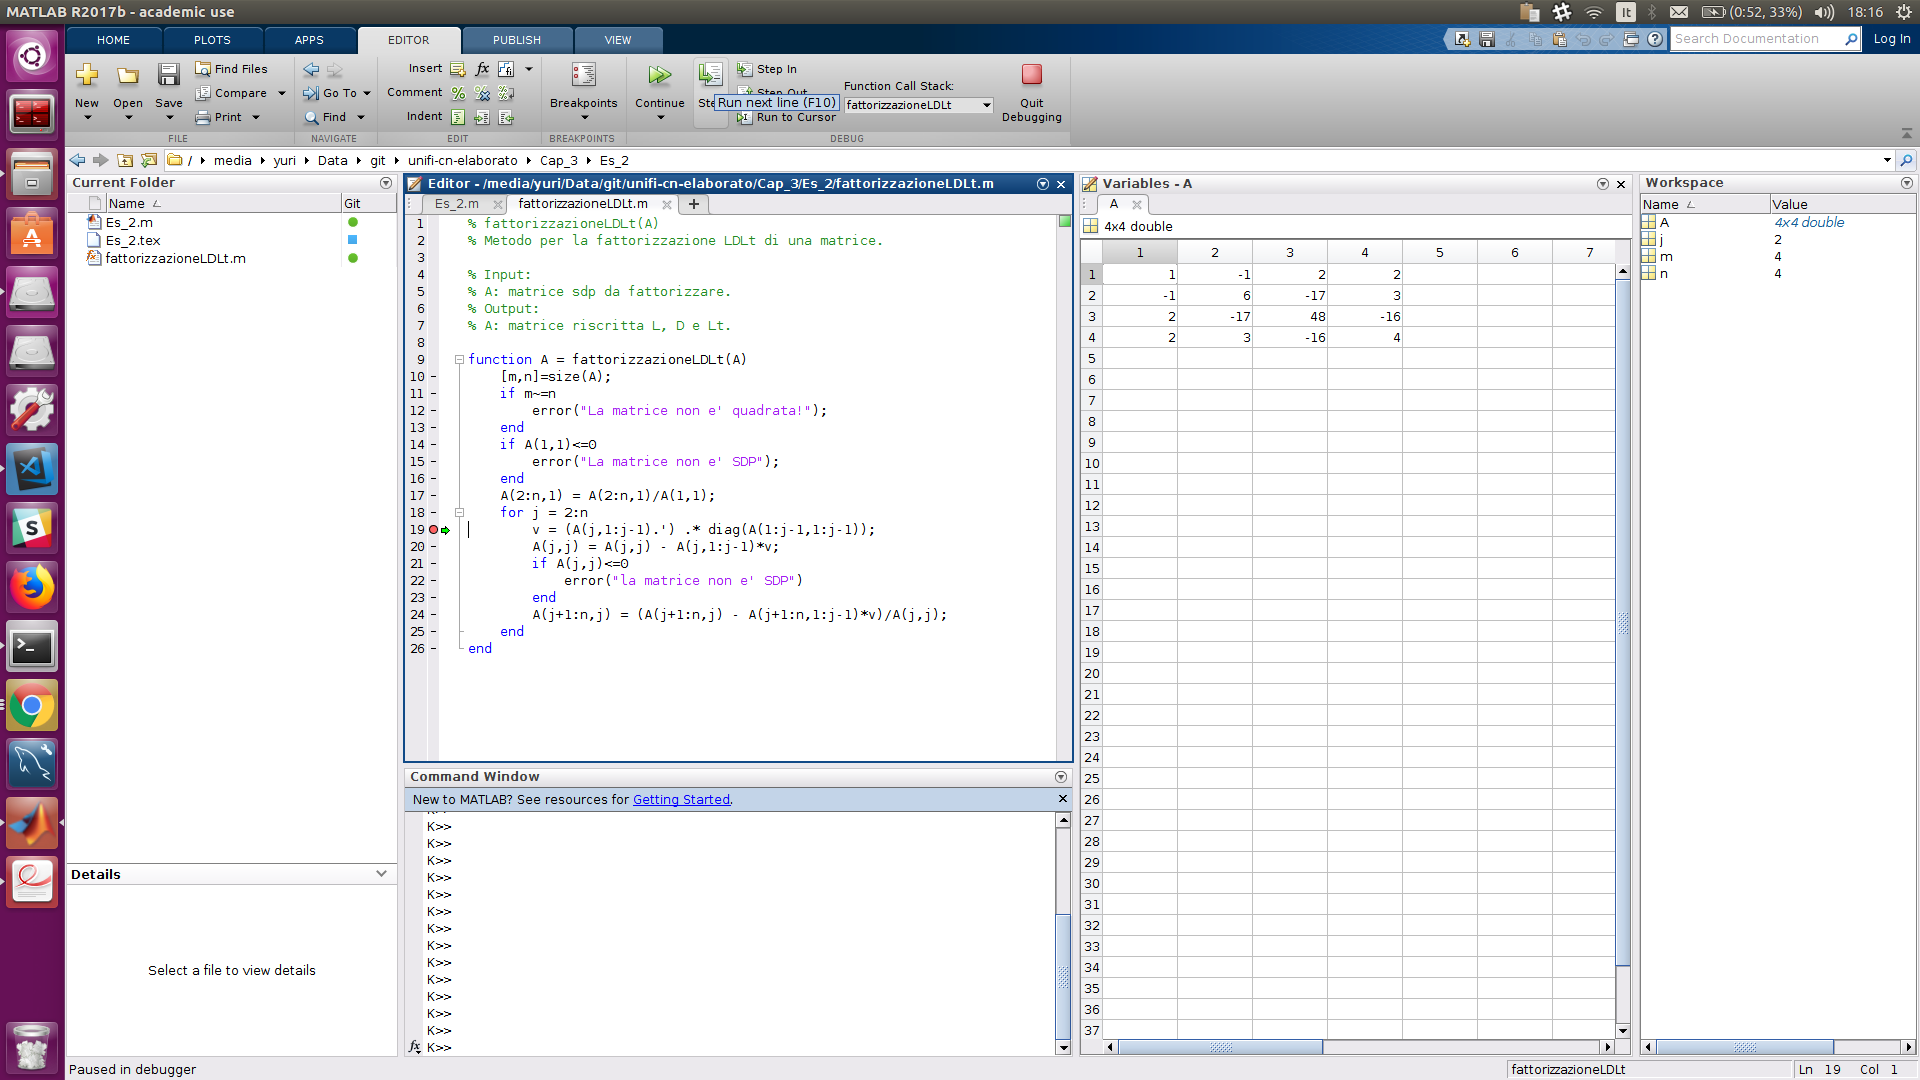
\includegraphics[width=\textwidth]{secondMatrix_0.png} \]
	      \[ 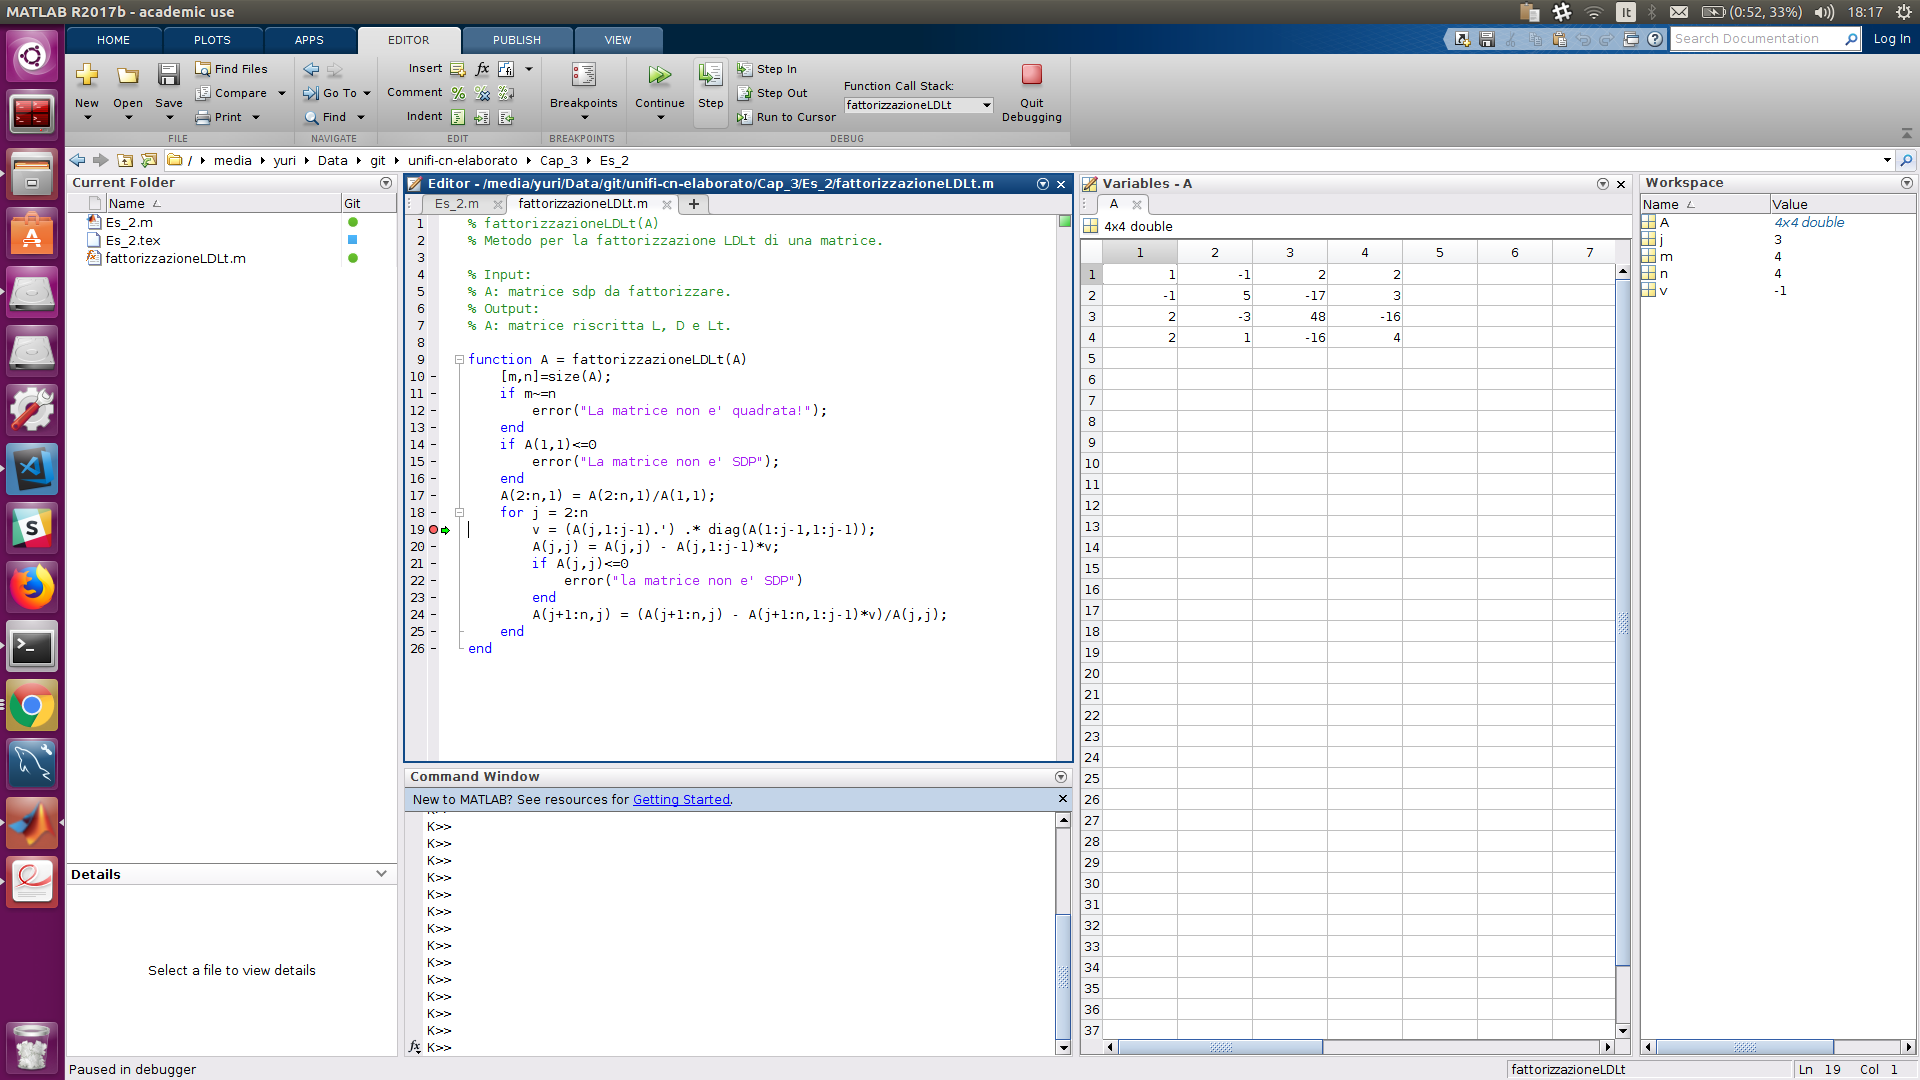
\includegraphics[width=\textwidth]{secondMatrix_1.png} \]
	      \[ 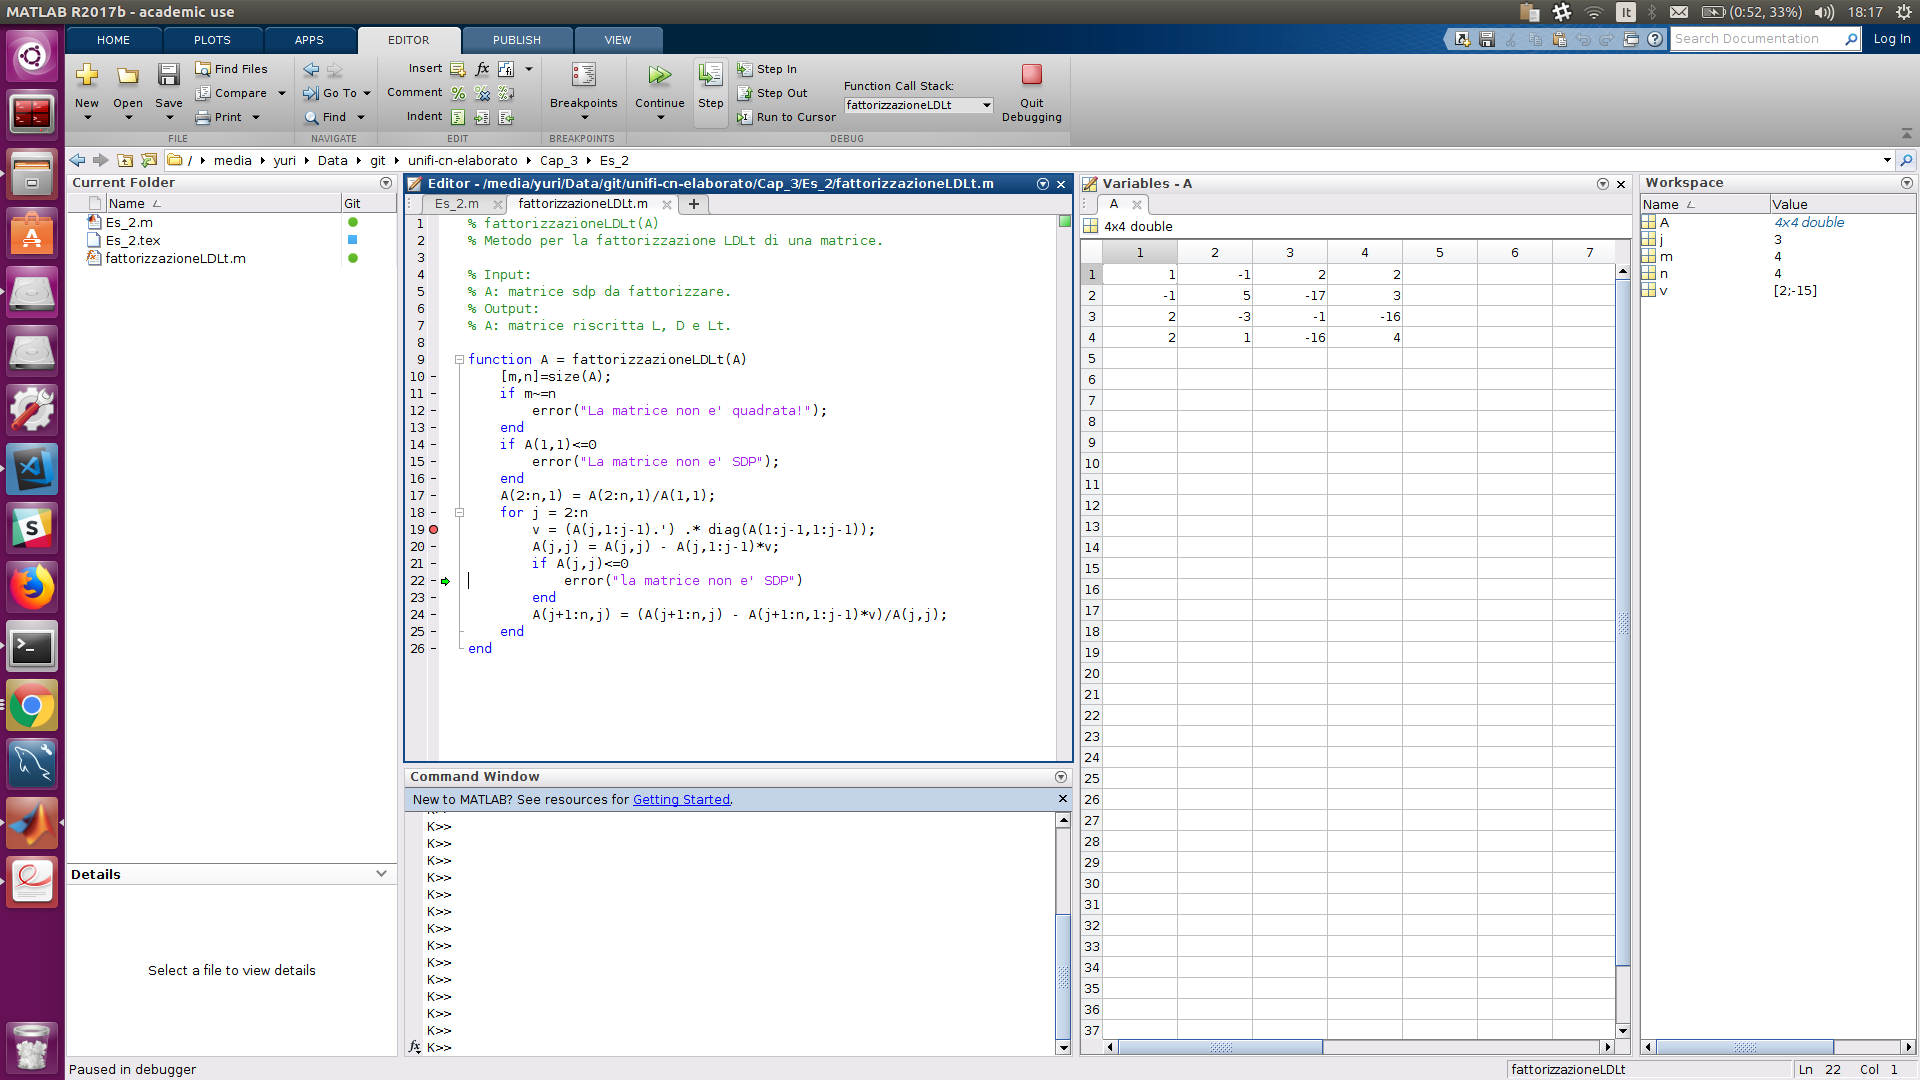
\includegraphics[width=\textwidth]{secondMatrix_2.png} \]
	      \end{enumerate}